\documentclass{prova}

\usepackage{amssymb}

\professor{Adriano Barbosa}
\disciplina{Ver\~ao 2024}
\avaliacao{de Geometria}
\curso{PROFMAT}
\data{05/02/2024}

\begin{document}
	\cabecalho{2}  % o numero 2 indica a qnt de quadros na tabela de nota
	\begin{questionario}
        \item Um recipiente cil\'{\i}ndrico de base circular est\'a parcialmente cheio de
            \'agua. Quando deitado, ou seja, apoiado sobre uma de suas geratrizes, o
            n\'{\i}vel da \'agua atinge um quarto do di\^anmetro $d$ da base do cilindro,
            confirme a figura abaixo. Quando o cilindro \'e levantado, isto \'e,
            apoiado sobre uma de suas bases, que fra\c{c}\~ao da altura $h$ do cilindro o
            n\'{\i}vel da \'agua atinge?
            \begin{figure}[h]
                \centering
                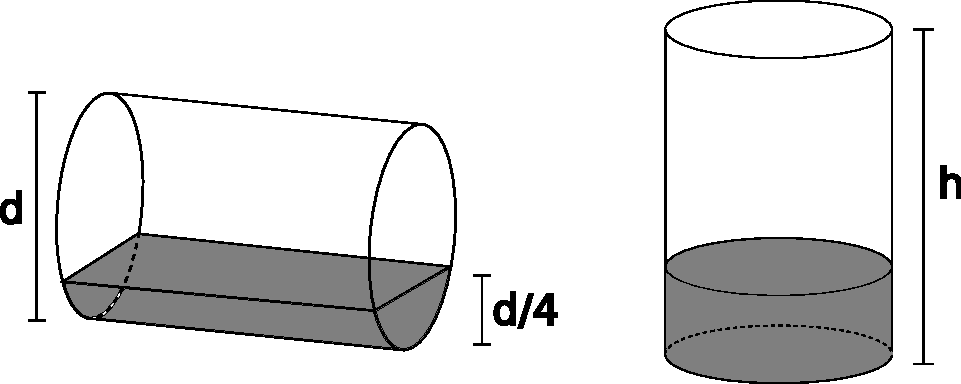
\includegraphics[width=0.6\textwidth]{fig01.pdf}
            \end{figure}

        \item A figura abaixo mostra um tri\^angulo equil\'atero e suas
            circunfer\^encias inscrita e circunscrita. A circunfer\^encia menor tem
            raio 1. Calcule a \'area da regi\~ao sombreada.
            \begin{figure}[h]
                \centering
                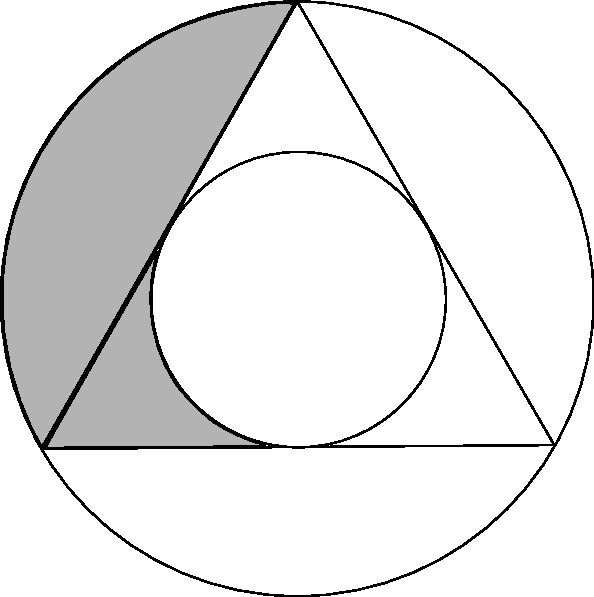
\includegraphics[width=0.3\textwidth]{fig02.pdf}
            \end{figure}
	\end{questionario}
\end{document}
